%%% demothesis.tex ---
%%
%% Filename: demothesis.tex
%% Description:
%% Author: Ola Leifler
%% Maintainer:
%% Created: Thu Oct 14 12:52:20 2010 (CEST)
%% Version: $Id$
%% Version:
%% Last-Updated: Wed Jun 28 10:57:24 2017 (+0200)
%%           By: Ola Leifler
%%     Update #: 169
%% URL:
%% Keywords:
%% Compatibility:
%%
%%%%%%%%%%%%%%%%%%%%%%%%%%%%%%%%%%%%%%%%%%%%%%%%%%%%%%%%%%%%%%%%%%%%%%
%%
%%% Commentary:
%%
%%
%%
%%%%%%%%%%%%%%%%%%%%%%%%%%%%%%%%%%%%%%%%%%%%%%%%%%%%%%%%%%%%%%%%%%%%%%
%%
%%% Change log:
%%
%%
%% RCS $Log$
%%%%%%%%%%%%%%%%%%%%%%%%%%%%%%%%%%%%%%%%%%%%%%%%%%%%%%%%%%%%%%%%%%%%%%
%%
%%% Code:

\documentclass[msc,lith,swedish]{liuthesis}
%% Settings go in settings.tex
%%% settings.tex ---
%%
%% Filename: settings.tex
%% Description:
%% Author: Ola Leifler
%% Maintainer:
%% Created: Tue Oct 19 21:11:31 2010 (CEST)
%% Version: $Id$
%% Version:
%% Last-Updated: Tue Apr 25 08:49:48 2017 (+0200)
%%           By: Ola Leifler
%%     Update #: 43
%% URL:
%% Keywords:
%% Compatibility:
%%
%%%%%%%%%%%%%%%%%%%%%%%%%%%%%%%%%%%%%%%%%%%%%%%%%%%%%%%%%%%%%%%%%%%%%%
%%
%%% Commentary:
%%
%%
%%
%%%%%%%%%%%%%%%%%%%%%%%%%%%%%%%%%%%%%%%%%%%%%%%%%%%%%%%%%%%%%%%%%%%%%%
%%
%%% Change log:
%%
%%
%% RCS $Log$
%%%%%%%%%%%%%%%%%%%%%%%%%%%%%%%%%%%%%%%%%%%%%%%%%%%%%%%%%%%%%%%%%%%%%%
%%
%%% Code:

\usepackage[backend=bibtex,sorting=none,style=numeric,natbib=true]{biblatex}
\usepackage{scrextend}
\usepackage{xifthen}
\usepackage{enumitem}
\usepackage{scrextend}
\newcounter{switchcase}

\newcommand{\ifequals}[3]{\ifthenelse{\equal{#1}{#2}}{\stepcounter{switchcase} #3}{}}
\newcommand{\case}[2]{#1 #2} % Dummy, so \renewcommand has something to overwrite...
\newenvironment{switch}[1]{
  %Executed at \begin{switch}
  \setcounter{switchcase}{0}
  \renewcommand{\case}{\ifequals{#1}}
}{
 % Executed at \end{switch}
\ifthenelse{\equal{\value{switchcase}}{0}}{
  \PackageError{ProjectDefinitions}{Could not find given definition}{}}{}
}

\newcommand{\definition}[1]
{
  \begin{switch}{#1}
    \case{Cachning}{\item [\textbf{#1}]
      Temporär lagning av data för snabb åtkomst.}
    \case{Instans}{\item [\textbf{#1}]
      En spelsession som startas från UI-applikationen och spelare kan gå med i för att spela spelet tillsammans.}
    \case{IoT-backend}{\item [\textbf{#1}]
      Existerande system som kan dirigera data mellan många uppkopplade enheter.}
    \case{Kontroll-applikation}{\item [\textbf{#1}]
      Applikation som körs på en mobil eller surfplatta och tar input från användare.}
    \case{Progressive Web Apps}{\item [\textbf{#1}]
      Förkortat PWA, är ett mellanting mellan en hemsida och en applikation.
      Med en PWA behöver man inte ladda ner en app, men den ger viss funktionalitet som appar har. \cite{bib-pwa}}
    \case{Resurs}{\item [\textbf{#1}]
      Media som används i spelet, t.ex. bilder och ljud.}
    \case{Sensor}{\item [\textbf{#1}]
      En sensor som sitter på kontroll-applikationen och inte är en pekskärm, t.ex. en accelerometer.}
    \case{Server-klient-modell}{\item [\textbf{#1}]
      Struktur på ett system där någon enhet tillhandahåller resurser, information eller tjänster och flera andra enheter interagerar med denna.}
    \case{Spelläge}{\item [\textbf{#1}]
      En utökning av grundspelet som definierar speciella regler och spelmekanik.}
    \case{Spelmekanik}{\item [\textbf{#1}]
      Regler och möjligheter som definierar ett spel.}
    \case{Tunn klient}{\item [\textbf{#1}]
      Specialfall av server-klient-modell där mycket få beräkningar sker på klienten.}
    \case{UI-applikation}{\item [\textbf{#1}]
      Applikationen som kör spelet och visar spelplanen.}
    \case{Use Case Map}{\item [\textbf{#1}]
      Diagram som illustrerar hur olika händelser interagerar med arkitekturen. \cite[p.~30--33]{bib-architecture-primer}}
    \case{Scrum-board}{\item [\textbf{#1}]
      En tavla med post-it lappar som innehåller aktiviteter som ska göras under
      projektet. Detta komplementeras med olika kolumner i tavlan såsom planerad, pågående,
      testning och utgåva. Dessa bestämmer i vilket stadie lapparna befinner sig i.}
    \case{Burndown-chart}{\item [\textbf{#1}]
      En graf som visar hur många timmar medlemmarna har lagt ner i förhållande till vad som krävs för att hinna med projektet.}
    \case{Acceptanstest}{\item [\textbf{#1}]
      Slutgiltiga testet som kund utför för att se att produkten lever upp till förväntningarna.}
    \case{Enhetstest}{\item [\textbf{#1}]
      Testa varje enhet så den fungerar när den är färdig.}
    \case{Integrationstest}{\item [\textbf{#1}]
      Testa att en ny enhet som läggs till i projektet fungerar som den ska tillsammans med de andra enheterna.}
    \case{Kund}{\item [\textbf{#1}]
      Cybercom Sweden.}
    \case{Regressionstest}{\item [\textbf{#1}]
      Testa ny kod enligt gamla parametrar för att säkerställa att ingen funktionalitet försvunnit.}
    \case{Systemtest}{\item [\textbf{#1}]
      Test för att säkerställa att enheten uppfyller kraven för projektet.}
    \case{Cybercom}{\item [\textbf{#1}]
      Kortare variant av Cybercom Sweden, företaget produkten utvecklas åt.}
    \case{Enkäten}{\item [\textbf{#1}]
      Den enkät som ska användas för att utvärdera användarupplevelsen, se avsnitt  3.3 Demo och enkät.}
    \case{Kvalitet}{\item [\textbf{#1}]
        I likhet med IEEE 730 definierar denna rapport kvalitet som konformitet till projektets krav. \cite{ieee730}}
    \case{Projektet}{\item [\textbf{#1}]
        Processen att framställa en produkt åt Cybercom Sweden.}
    \case{Software Quality Asssurance}{\item [\textbf{#1}]
    	Förkortat SQA, är en samling aktiviteter som bedömmer lämpligheten och inger förtroende
    	för utvecklingsmetodiken som används.}
    \case{SQA-process}{\item [\textbf{#1}]
      I likhet med IEEE 730 definieras en SQA-process som aktiviteten att samla underlag för att med säkerhet ta
      beslutet av produkten uppnår sina kvalitetskrav}
    \case{Teamet}{\item [\textbf{#1}]
      Det team av åtta studenter som tillsammans ska utföra projektet}
    \case{Trello}{\item [\textbf{#1}]
      En hemsida för att lägga till och fördela uppgifter bland flera personer, kan liknas till en whiteboard som
      postit lappar fästs på.}
    \case{Speldata}{\item [\textbf{#1}]
      Information om handlingar och status i spelet samt nödvändig teknisk data för
      att upprätthålla kommunikation.}
    \case{Realtidsmultiplayerspel}{\item [\textbf{#1}]
      Spel där flera användares handlingar har en direkt inverkan på spelets tillstånd.}
    \case{Gamemode}{\item [\textbf{#1}]
      En variant av basspelet med eventuellt andra funktioner och regler.}
    \case{Vanliga nätverksförhållanden}{\item [\textbf{#1}]
      En enhet med en stabil internetuppkoppling utan yttre störningar.}
    \case{React}{\item [\textbf{#1}]
      Javascript-bibliotek för att bygga hemsidor och mer avancerade webbsystem.\cite{bib-react}}
    \case{Deep Stream}{\item [\textbf{#1}]
    Kommunikationssystem som tillåter synkronisering av data mellan många enheter i realtid. Tillgängligt i många olika programmeringsspråk, bland annat javascript.\cite{bib-deepstream}}
    \case{Impact Map}{\item [\textbf{#1}]
    Diagram som visar inverkan av händelser under ett mjukvarusystems livstid. Kan visa på effekterna av implementation av ny funktionalitet, fel i systemet eller säkerhetsintrång.\cite[p.~91--93]{bib-architecture-primer}}
    \case{IoT, Internet of things}{\item [\textbf{#1}]
    Internet of things -- Ett begrepp som beskriver den tekniska och samhälleliga utveckling då fler och fler saker blir uppkopplade mot internet.}
    \case{Gitrepo}{\item [\textbf{#1}]
    En datastruktur för att lagra och hantera olika versioner av kod i git.}
    \case{Master-branch}{\item [\textbf{#1}]
    Standardgrenen till ett gitrepo som vanligtvis reflekterar repot i ett fungerande tillstånd.}
	\case{Kursen}{\item [\textbf{#1}]
    Den kurs som detta projekt utförs inom, det vill säga LiTHs kurs ''Kandidatprojekt i programvaruutveckling'' med kurskod TDDD96}
  \case{npm}{\item [\textbf{#1}]
  Node Package Manager -- En pakethanterare för Javascripts ekosystem}
  \case{npm-paket}{\item [\textbf{#1}]
  Ett paket med Javascript-kod som finns tillängligt i npm}


  \end{switch}
}

\setlength\parindent{0pt}
\parskip = \baselineskip

%% To set the font of your thesis, use the \setmainfont{} command,
%% surrounded with \ifxetex if you want to switch between xelatex and pdflatex
\ifxetex
%\setmainfont [Scale=1]{Georgia}
\fi

%%%%%%%%%%%%
%% The VZ43 chapter style, from Memoir contributed chapter styles: ftp://ftp.tex.ac.uk/ctan%3A/info/MemoirChapStyles/MemoirChapStyles.pdf
%%%%%%%%%%%

\setcounter{secnumdepth}{3}

\usepackage{calc,color}
\newif\ifNoChapNumber
\newcommand\Vlines{%
\def\VL{\rule[-2cm]{1pt}{5cm}\hspace{1mm}\relax}
\VL\VL\VL\VL\VL\VL\VL}
\makeatletter
\setlength\midchapskip{0pt}
\makechapterstyle{VZ43}{
\renewcommand\chapternamenum{}
\renewcommand\printchaptername{}
\renewcommand\printchapternum{}

\renewcommand\chapnumfont{\Huge\bfseries\centering}
\renewcommand\chaptitlefont{\Huge\bfseries\raggedright}
\renewcommand\printchaptertitle[1]{%
\Vlines\hspace*{-2em}%
\begin{tabular}{@{}p{1cm} p{\textwidth-3cm}}%
\ifNoChapNumber\relax\else%
\colorbox{black}{\color{white}%
\makebox[.8cm]{\chapnumfont\strut \thechapter}}
\fi
& \chaptitlefont ##1
\end{tabular}
\NoChapNumberfalse
}
\renewcommand\printchapternonum{\NoChapNumbertrue}
}
\makeatother

%% To set bibliography options, refer to the biblatex manual and use
%% the ExecuteBibliographyOptions command below to set your options

\ExecuteBibliographyOptions{maxnames=99}


%% Change this to your appropriate BibTeX reference file (.bib)

\addbibresource{../references.bib}
\addbibresource{individuall/joel_o/joel_o-references.bib}

\usepackage{rotating}
\usepackage{color}

% \usepackage{changebar}

\department{Institutionen för datavetenskap}
\departmentenglish{Department of Computer and Information Science}
\departmentshort{IDA}
% If this is a thesis at the cognitive science study programme, use
% the "area" command to generate a proper (?) ISRN
% \area{KOGVET-A}

% Include an external supervisor on the cover page
% \externalsupervisor{Min företagshandledare}
\supervisor{Carl Brage}
\examiner{Kristian Sandahl}
\titleenglish{Realtime Multiplayer Game on IoT-Backend}
\subtitleenglish{with a subtitle}
\titleswedish{Realtidsultiplayerspel på IoT-Backend}
\thesissubject{Datateknik}

\publicationyear{2018}
\currentyearthesisnumber{001}
\dateofpublication{2015-05-08}

\author{Författaren}

% Two authors
% \author{\parbox{\textwidth}{Ola Leifler\\
%   Alexander Sanner}}

\begin{document}

\chapterstyle{VZ43}

\chapter{Introduktion}
\label{cha:introduction}

Detta projekt utfördes som en del av kursen ''Kandidatprojekt i Programvaruutveckling'' på LiTH våren 2018. Det genomfördes av en grupp studenter som går civilingenjör i datateknik samt civilingenjör i mjukvaruteknik.
Denna introduktion är uppdelad i fyra delar som tillsammans framför vad denna rapport kommer att gå igenom.

\section{Motivering}
\label{sec:motivation}
Trenden Internet of Things (IoT) har blivit mer populär den senaste tiden\cite{IoT-ecosystem}, och fler aktörer har möjligheten att koppla upp sin verksamhet till internet. Utrustning kan kopplas till IoT av många olika anledningar, till exempel kan fabriker använda sig av IoT för att få en bättre överblick av slitaget på sina maskiner. För privatpersonen kan produkter kopplas till IoT såsom ett kylskåp där innehållet kan ses genom en smarttelefon. En central del i IoT är hur slussandet av data sker, för det måste hamna på rätt ställe samtidigt som det ska gå snabbt. Storleksordningen av dessa egenskaper för ett bra resultat är dock inte genomskinligt för en person som inte är insatt i området. Därför gavs gruppen uppdraget att skapa ett interaktivt system för att demonstrera responsiviteten hos Cybercoms IoT-system. Detta system är ett realtidsspel där spelarens handlingar omgående påverkar dennes pjäs på spelplanen, samtidigt som datan går igenom Cybercoms IoT-servrar.


\section{Frågeställning}

\begin{enumerate}
	\item \label{fs:fs_1} Hur kan ett realtidsspel som använder sig av Cybercoms backend implementeras så att man skapar värde för kunden?
	\item \label{fs:fs_2} Vilka erfarenheter kan dokumenteras från programvaruprojektet som kan vara intressanta för framtida projekt?
	\item \label{fs:fs_3} Vilket stöd kan man få genom att skapa och följa upp en systemanatomi?
	\item \label{fs:fs_4} Hur kan kontinuerliga användardemonstrationer användas i utvecklingsfasen för att förbättra ett spels kvalitet?

\end{enumerate}

\section{Syfte}
\label{sec:aim}
Syftet med denna rapport är att dokumentera erfarenheter som teamet har fått genom processen av produktens utveckling, samt projektets utförande. Dessutom så
 har rapporten som syfte att utreda hur utvecklingen av ett realtidsmultiplayerspel skapar värde för kunden, och eventuellt möta deras behov av att testa hastigheten samt skalbarheten hos kundens backend.


Projektets syfte är att skapa ett realtidsmultiplayerspel för att demonstrera hastigheten, responsiviteten, och skalbarheten på Cybercom IoT-backend vilket görs på deras begäran.
\section{Avgränsning}
\label{sec:delimitations}

Projektet utförs som en del av kursen ''Kandidatprojekt i Programvaruutveckling''. Detta innebär att projektet har en begränsad tidsbudget på 400 timmar
per gruppmedlem, det vill säga 3200 timmar totalt. Kursen innefattar obligatoriska seminarier, föreläsningar, workshops och dokumentskrivning som också är inräknade i tidsbugeten.
Projektet utför en testning av Cybercoms backend och därför är projektet direkt beroende av backendens funktionalitet.

\chapter{Teori}
\label{cha:theory}
I detta avsnitt beskrivs grundläggande teoretiska begrepp och ramverk som följdes under projektets gång. Här beskrivs de essentiella programmeringsverktyg och ramverk för projektet samt utvecklingsmetoden Scrum. 
\section{Utvecklingsverktyg för produkt}
Det här avsnittet redovisar vilka verktyg projektgruppen har använt för att utveckla produkten samt hur projektgruppen har använt sig av dessa verktyg.

\subsection*{React}
Ramverket React användes för att utveckla UI-applikationen samt kontroller-applikationen. Ett krav från kunden var att produkten skulle skrivas i JavaScript. React är ett Javascript bibliotek som bidrar med mycket funktionallitet vilket underlättar utvecklandet av användargränssnittet.  Detta bestämdes tidigt i projektet då vissa projektmedlemmar hade tidigare erfarenheter med React ramverket \cite{ReactAJa67:online}.

\subsection*{Yarn}
Yarn är ett Javascript bibliotek. Biblioteket fungerar som en pakethanterare som skapar beroende mellan paket och underhåller dessa. Detta gör det enklare att lägga till och ta bort bibliotek till ett projekt \cite{GettingS85:online}.

\subsection*{Prettier}
Prettier är ett verktyg för att formatera kod på ett standardiserat och lättläsigt sätt\cite{prettier}. Prettier går igenom koden och lägger till eller tar bort blanksteg och nya rader enligt förutbestämda regler. Syntaktiskt blir koden samma före och efter att Prettier körts, men läsbarheten lär ha förändrats. Prettier tar även bort stilpreferenser som olika kodskribenter då den alltid formaterar koden enligt samma regler.


\subsection*{Eslint}
Eslint är ett \textit{open source} program som definerar stilregler för hur Javascriptkod skrivs. Dessa stilregler handlar  om hur kod ska formateras och att följa bra programmeringspraxis. Eslint söker sen igenom koden för rader som bryter mot de satta reglerna och påpekar alla fall som deta sker. Oftast så integreras Eslint in till programet där koden skrivs för att få Eslints varningar direkt när koden skrivs. De regler Eslint efterföljer är bra praxis för kodning i Javascript och de går att ändra på efter behov.


\subsection*{Node.js}
Node.js är en exekveringsmiljö för Javascript. Nodes.js ger funktionallitet att emulera en server med sin applikation på lokalt på sin dator \cite{Nodejs11:online}. Att Node.js skulle användas var ett krav från kunden.

\subsection*{PIXI}
PIXI är ett kraftfullt \textit{opensource} renderingsbiblotek för Javascript\cite{PixiJSv473:online}. Den erbjuder funktioner som att rendera geometriska former och bilder samt en uppdateringsloop varje gång ett objekt ritas ut igen. PIXI är väldigt populärt och används av många stora företag såsom Google, Ubisoft och Spotify. 

\subsection*{Scrum}
Scrum är en populär agil utvecklingsmetodik inom mjukvaruutveckling. Metoden är anpassad för en mindre grupp på 5-9 medlemmar. Scrum använder ett iterativt, inkrementellt tillvägagångssätt som är relevant för detta projekt då den tillåter ändringar att ske när det behövs\cite{TheScrum81:online}. I Scrum delas arbetet i mindre iterationer kallas för \textit{sprint}. En sprint kan vara 1-4 veckor lång. Varje sprint planeras vid dess början och då bestäms mål som ska vara färdiga vid sprintensslut. Efter en sprint så utvärderas hur väl arbetet gick under denna sprint samt vad som bör göras annorlunda till nästa sprint. Scrum har många inslag som är typiska för just Scrum, de som tas upp i denna rapport är följande:

\begin{itemize}
	\item \textit{Scrum-bräde} är ett bräde med alla uppgifter som ska göras under en sprint, varje medlem kan sedan ta en egen uppgift och flytta den till rätt kategori beroende på hur det går i arbetet med den. Vanliga kategorier är: att göras, pågående, testing, färdig.
	
	\item \textit{Burndown chart} är en graf som visar kvarstående arbetet. Grafen hjälper teamet att ta reda på om de ligger bra eller dåligt till för att leverera dem uppgifter som de har åtagit sig. 
	
	\item \textit{Produkt-backlog}: En lista av prioriterade önskemål som visar vad kundens önskemål vid slutprodukten.
	
	\item \textit{Sprint-backlog} nedbrutna uppgifter ifrån produkt-backlogen som teamet åtar sig att leverera under en sprint. 	
	
\end{itemize}

\subsection*{Trello}
Trello är en hemsida för att skapa och fördela uppgifter bland flera personer. Det kan liknas till en anslagstavla där lappar med uppgifter kan klistras på. Anslagstavlan i sig är uppdelad i kategorier som användarna själva kan skapa och modifiera. Oftast så har dessa kategorier namn som att ''att göra'', ''pågående'' och ''färdigt''. Lappar fästs sen vid den första kategorien ''att göra'' och flyttas sedan till de andra när det anses passande. Varje lapp har sedan möjlighet att innehålla extra information bland annat: vem som arbetar med den, en beskrivning av lappen samt en tidsuppskattning. Alla fält på en lapp bortsett dess namn är friviliga, och därav så kan en Trello-lapp innehålla väldigt mycket, eller väldigt lite, information.

\subsection{Git}
Ett opensource projekt som används för versionhantering av kod \cite{Git52:online}.
\begin{itemize}
	\item \textit{Push}: Skickar utvecklingsfiler från det lokala repot som man utvecklar i till Gitrepot.
	\item \textit{Pull request}: En begäran som skickas när en utvecklare laddar ner en kod från Git, modiferar den och vill \textit{pusha} tillbaka den. När en pull request är gjord intresserade partier kan se över modifieringar som har gjorts och sammanfoga den i huvudgrenen, begära ytterligare modifieringar, eller pushar egna modifieringar. 
	\item \textit{Gren}: En oberoende utvecklingslinje som en utvecklare kan uttnytjan när hen vill lägga till nya funktionalitet. 
\end{itemize}

\subsection*{Github}
Github är en hemsida som integrerar Git och tillåter användare att lägga upp sin kod där gratis förutsatt att den är offentlig. Github erbjuder även en visualisering av många av Gits funktionaliteter såsom en grafisk vy över hur koden förändrats över tid eller skillnaderna mellan två versioner. Github erbjuder även verktyg för att strukturera ett projekt såsom möjligheten att enkelt bjuda in medlemmar och ändra hur vilka rättigheter de ska ha. Dessa rättigheter kan vara allt mellan att inte ha tillgång till någon förändring till att få ändra all kod i alla grenar. Github möjliggör också för integration med Travis på sin plattform. Dess primära funktionen är dock en att tillhandahålla ett Gitrepo på en server för att minimera risken av förlorat arbete vid en krash.

\subsection*{Travis}
Ett opensource testningstjänst som erbjudst av gratis Github på deras plattform. Travis används i kontinuerlig integration för att köra tester på alla grenar innan de kan mergeas in i huvudgrenen.

\subsection*{Slack}
Slack är ett kommunikationsverktyg som ofta används proffesionelt inom IT och mjukvaruutveckling. Funktionsmässigt är det ett chatprogram för datorer och mobila enheter.

\subsection*{Latex}
Latex är ett gratis verktyg som kombinerat med en latex-editor används för att skapa artiklar och rapporter av olika slag. Det är ett väldigt kraftigt verktyg som med många formateringsmmöjligheter och tillskillnad ifrån många andra text-editors så separerar Latex mellan det du skriver och slutprodukten som ska läsas.

%%% lorem.tex ---
%%
%% Filename: lorem.tex
%% Description:
%% Author: Ola Leifler
%% Maintainer:
%% Created: Wed Nov 10 09:59:23 2010 (CET)
%% Version: $Id$
%% Version:
%% Last-Updated: Wed Nov 10 09:59:47 2010 (CET)
%%           By: Ola Leifler
%%     Update #: 2
%% URL:
%% Keywords:
%% Compatibility:
%%
%%%%%%%%%%%%%%%%%%%%%%%%%%%%%%%%%%%%%%%%%%%%%%%%%%%%%%%%%%%%%%%%%%%%%%
%%
%%% Commentary:
%%
%%
%%
%%%%%%%%%%%%%%%%%%%%%%%%%%%%%%%%%%%%%%%%%%%%%%%%%%%%%%%%%%%%%%%%%%%%%%
%%
%%% Change log:
%%
%%
%% RCS $Log$
%%%%%%%%%%%%%%%%%%%%%%%%%%%%%%%%%%%%%%%%%%%%%%%%%%%%%%%%%%%%%%%%%%%%%%
%%
%%% Code:

\chapter{Method}
\label{cha:method}
Det här kapitlet beskriver hur projektet har utförts samt beskrivningar av de metoder och verktyg som använts för de olika områden projektet omfattar.

\section{Projekt organisation}
Det här avsnittet förklarar hur projektgruppen är strukturerad. Avsnittet beskriver även vilka metoder och verktyg som har använts för att sköta den interna kommunikationen och förklarar utvecklingssmetodiken projektgruppen har följt.

\subsection{Roller}
Projektetgruppen är strukturerad av förbestämda roller. Varje gruppmedlem tilldelades en roll vid projektetsstart efter en intern valprocess. Rollerna är väldefinierade och dess ansvarsområden.

\subsubsection*{Teamledare}
Teamledaren ska se till att samtliga processer som ska utföras under projektets gång följs. Denna person representerar också teamet utåt och har kontakt med handledaren. Om det behövs har teamledaren sista ordet.

\subsubsection*{Kvalitetssamordnare}
Kvalitetssamordnaren ansvarar för arbetsprocesser som ska hålla kvaliten av projektet på en hög nivå. Samordnaren gör en budget av vad kvalitet får kosta, samtidigt som han ansvarar för kvalitetsplanen.

\subsubsection*{Dokumentansvarig}
Dokumentansvarig ser till att ansvara för samtliga dokument som teamet ska producera. Även ansvarig för gruppens logotyp och dokumentmallar.

\subsubsection*{Arkitekt}
Arkitekten ansvarar för arkitekturen av den tekniska delen av projektet. Gör övergripande teknikval och har det sista ordet på tekniska beslut.

\subsubsection*{Utvecklingsledare}
Utvecklingsledaren ansvarar för den mer detaljerade designen av den tekniska produkten. Leder utvecklingsarbetet och ser till att resten av teamet har något att arbeta med.

\subsubsection*{Analysansvarig}
Analysansvarig ansvarar för majoriteten av kundkontakt och jobbar ständigt med att ta reda på kundens verkliga behov. Har huvudansvar för kravspecifikationen.

\subsubsection*{Testledare}
Testledaren beslutar systemets status genom att arbeta tillsammans med kvalitetssamordnaren för att testa så systemet uppnår kraven. Skriver testplan och testrapport.

\subsubsection*{Konfigurationsansvarig}
Konfigurationsansvarig ansvarar för generell versionshantering i projektet. Arbetar mycket med utvecklingledaren och dokumentansvarig för att bestämma vilka arbetsprodukter som ska ingå i en utgåva.

\section{Utvecklingsmetodik}

\subsection{Projektfaser}
Projektet uppdelades i 4 iterationer.

\subsubsection*{Förestudier}
\subsubsection*{Utveckling}
\subsubsection*{???}
\subsubsection*{???}

\subsection{Sprint}
Trello användes för att organisera varje sprint i projektet. Ett trello-board för en sprint bestod av kolumerna TODO, currently doable, in progress, stalled och done. Under TODO hamnade alla aktiviteter projektgruppen kunde producera, aktiviteter kunde läggas till denna kolumn under en pågående sprint. TODO kolumnen kan liknas med en product backlog i Scrum. I kolumnen currently doable hamnade alla aktiviter som förväntades bli klara till en sprints slut. Varje aktivitet bestod av två attribut, prioritet och tidsestimering. Dessa attribut sattes när en sprint planerades och hjälpte gruppen att belasta varje sprint med en bra mängd aktiviteter. Under rubriken in progress hamnade alla aktiviteter som en eller flera projektmedlemmar arbetade med. I stalled kolumnen hamnade alla aktiviterer som påbörjats men pausats på grund av andra prioriteringar. I Done kolumnen hamnade alla aktiviteter som blvit avklarade. Kolumnen användes för att utvärdera sprinten och fungerade som en log över vad som hade gjorts.

\subsection{Testning}


\subsection{Möten}
En gemensam Google kalender skapades där alla möten samt viktiga moment lades till.

\subsection{Utbildning}

\subsection{Kommunikation}
Kommunikationen mellan externa parter och projektgruppen gick i huvudsak genom rollerna team ledare och analysansvarig. Slack användes för både den interna- och externa kommunikationen under projektetsgång. En Slack arbetsplats skapades, där enbart projektgruppen var medverkande i, skedde majoriteten av all den interna kommunikationen. Olika kanaler skapades på denna Slack arbetsplats för att diskutera olika ärenden och hålla kommunikationen strukturerad. Det fanns ytterligare en slack arbetsplats där både projektgruppen och kunden medverkade i, på denna arbetsplats skedde majoriteten av den externa kommunikationen med kunden. Även denna arbetsplats var uppdelad i olika kanaler, frågor och allmänt. Tanken bakom frågor kanalen var att projektgruppen kunde fylla kanalen med frågor rörande utvecklingen och kunden kunde bearbeta frågorna när de hade tid. Allmänt kanalen användes för all övrig kommunikation.

\subsection{Versionshantering}

\section{Dokumentation}
Det här avsnittet beskriver vilka verktyg som har använts för att dokumentera projektgruppens arbete samt vilka dokument som har producerats och dess syften.

\subsubsection*{Projektplan}
Projektplan består av en beskrivning utav projektet, 
resurser som teamet har tillgång till, processer som kommer användas och risker inom projektet.
Dessutom beskrivs en aktivitetsplan som översiktligt tar upp alla aktiviteter som kommer att
göras under projektet.

\subsubsection*{Kravspecifikation}
Kravspecifikationen förtydligar vad som förväntas vara klart vid projektets slut. Dokumentet fungerar som överenskommelse mellan kunden och projektgruppen. Kraven specificerar vilken funktionallitet, kvalitet och design produkten ska uppfylla. Dokumentet utgör grunden för hur hela projektet ska struktureras och utformas. Kraven är framtagna efter kundens önskemål och formulerade för att ligga till stöd för projektgruppensarbete.

\subsubsection*{Kvalitetsplan}
Kvalitetsplanen definierar processer vars syften är att säkerställa att produkten håller en hög kvalitet. Kvaliteterna som är i huvudfokus är definerade i kravspecifikationen och är baserade på kundens önskemål.

\subsubsection*{Statusrapport}
Statusrapporten är som en mindre projektplan för
de olika iterationerna. Rapporten reflekterar över hur allt förarbete har gått, vad som kommer
hända till nästa iteration samt vilka risker projektgruppen står inför.

\subsubsection*{Systemanatomi}
Anatomin för systemet beskriver hur systemet är uppbyggt på olika nivåer, såsom funktioner, 
mjukvara, hårdvara. Anatomin ger en större bild för hur systemet fungerar och beskriver vilken miljö den kommer
befinna sig i.

\subsubsection*{Arkitekturbeskrivning}
Arkitekturbeskrivningen detaljerar arkitekturen för systemet samt beskriver hur olika submoduler hänger ihop. Arkitekturens fördelar, nackdelar och möjliga utökningar förklaras även i dokumentet.

\subsubsection*{Testplan}
Testplanen beskriver hur de olika delarna av produkten ska testas och även hur man ska följa upp på testerna.

\subsubsection*{Gruppkontrakt}
Projektgruppen producerade och undertecknade ett gruppkontrakt[gruppkontrakt] som skrevs vid ett tidigt stadie för att förtydliga vad som förväntades av varje gruppmedlem.

\subsubsection*{Tidrapport}
Tidrapporteringen under projektet skedde i ett excelblad där varje teammedlem rapporterade den tid de har spenderat under en dag. Tiderna som skrevs in fick inte överstiga två timmar och arbetspass som varade längre skrevs som två olika arbetstillfällen. I och med detta kunde även ett burndown-chart genereras för att få en bättre uppfattning om hur teamet ligger till i tidsåtgång.

\subsubsection*{Mötesprotokoll}
Under projektet hölls olika möten för att diskutera saker som har kommit upp. Dessa behövdes dokumenteras vilket gjordes med hjälp av en mötesprotokollmall som fylldes ut under varje möten.

\subsection{Dokumentlagring}
Dokumenten som skapades under projektets gång lagrades på Google Drive för att både versionshantera de olika färdiga iterationerna av dokumenten, men även för att enkelt kunna se dokumenten om LaTeX inte finns till hand. Dessutom versionshanterades dokumenten under arbetets gång med hjälp av git genom GitHub. Detta hjälpte dokumentskrivning genom att hantera olika konflikter när olika personer sitter i samma fil och skriver. 

\subsection{Dokumentskrivning}
Själva dokumentskrivningen utfördes genom att skriva i LaTeX, vilket gjorde det lättare att dela upp dokumenten i olika sektioner.   

\section{Metod för att fånga erfarenheter}



%%%%%%%%%%%%%%%%%%%%%%%%%%%%%%%%%%%%%%%%%%%%%%%%%%%%%%%%%%%%%%%%%%%%%%
%%% lorem.tex ends here

%%% Local Variables:
%%% mode: latex
%%% TeX-master: "demothesis"
%%% End:

%%% lorem.tex ---
%%
%% Filename: lorem.tex
%% Description:
%% Author: Ola Leifler
%% Maintainer:
%% Created: Wed Nov 10 09:59:23 2010 (CET)
%% Version: $Id$
%% Version:
%% Last-Updated: Wed Nov 10 09:59:47 2010 (CET)
%%           By: Ola Leifler
%%     Update #: 2
%% URL:
%% Keywords:
%% Compatibility:
%%
%%%%%%%%%%%%%%%%%%%%%%%%%%%%%%%%%%%%%%%%%%%%%%%%%%%%%%%%%%%%%%%%%%%%%%
%%
%%% Commentary:
%%
%%
%%
%%%%%%%%%%%%%%%%%%%%%%%%%%%%%%%%%%%%%%%%%%%%%%%%%%%%%%%%%%%%%%%%%%%%%%
%%
%%% Change log:
%%
%%
%% RCS $Log$
%%%%%%%%%%%%%%%%%%%%%%%%%%%%%%%%%%%%%%%%%%%%%%%%%%%%%%%%%%%%%%%%%%%%%%
%%
%%% Code:

\chapter{Resultat}
\label{cha:results}

Detta kapitel tar upp de resultat som projektgruppen kommit fram till under projektets gång.

\section{Systembeskrivning}

Projektgruppen definierade en tydlig design av applikationen innan implementationen påbörjades. Detta var för att försäkra sig om att applikationen skulle bli av hög kvalitet och eventuella designproblem skulle hittas tidigt i projektet.

\subsection{Systemanatomi}
\label{beskrivning-systemanatomi}
Under iteration ett producerade projektgruppen en systemanatomi av applikationen som skulle utvecklas. Denna producerades utifrån de use-cases och krav kunden hade tillhandahållit. I figur \ref{fig:systemanatomi_graf} visas systemanatomin för hela systemet och i \ref{fig:systemanatomi_spel} visas den för själva spelet.

\begin{figure}[H]
    \centering
    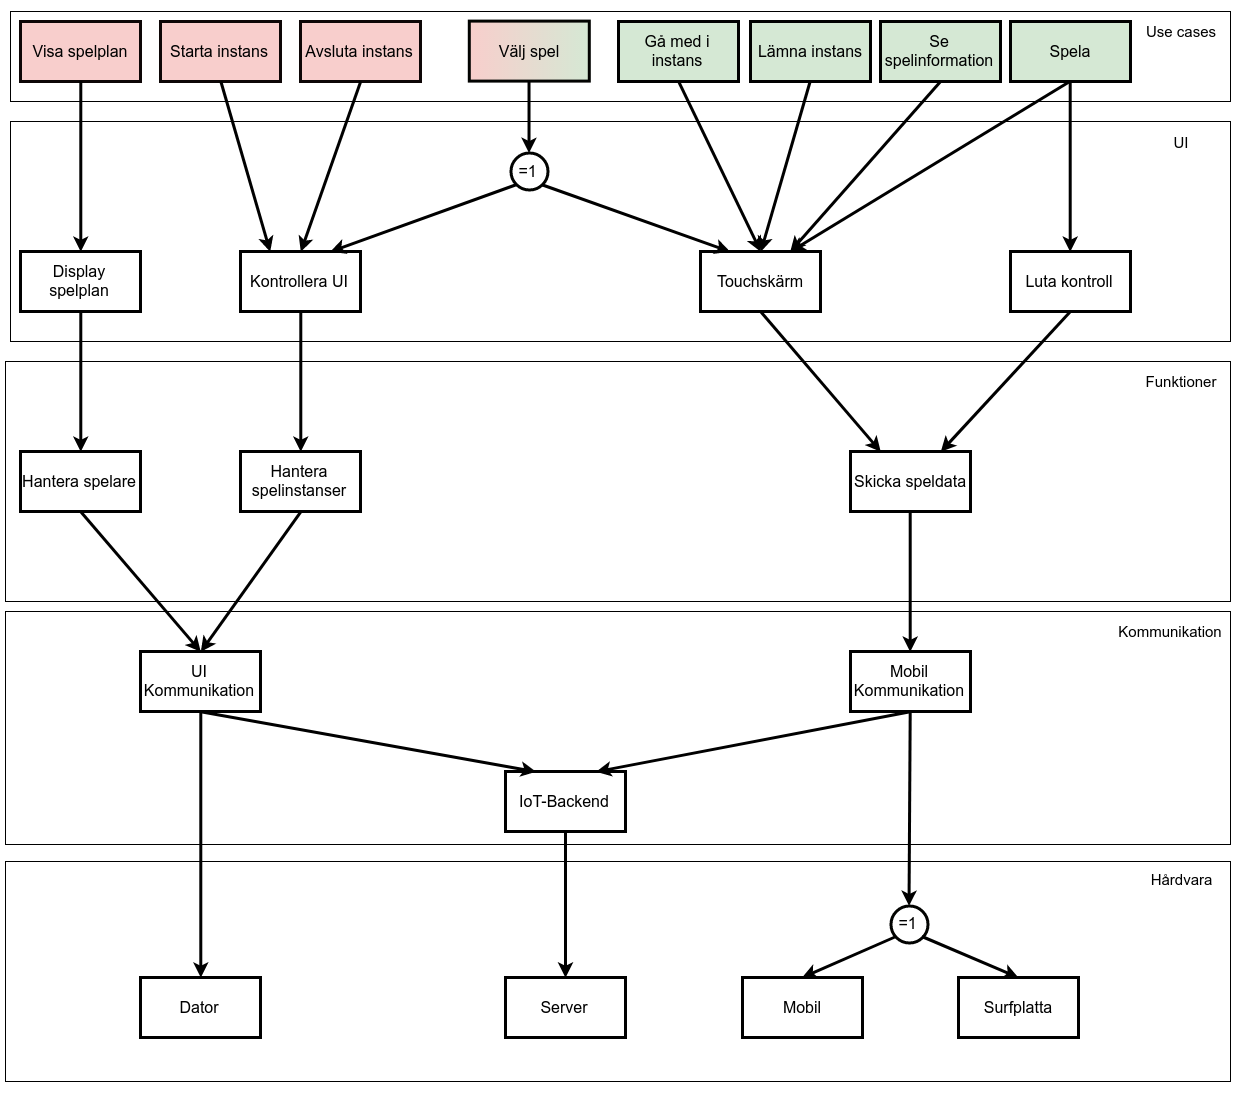
\includegraphics[scale=0.3]{systemanatomi_graf}
    \caption{Överblick av systemanatomin}
    \label{fig:systemanatomi_graf}
\end{figure}

\begin{figure}[H]
    \centering
    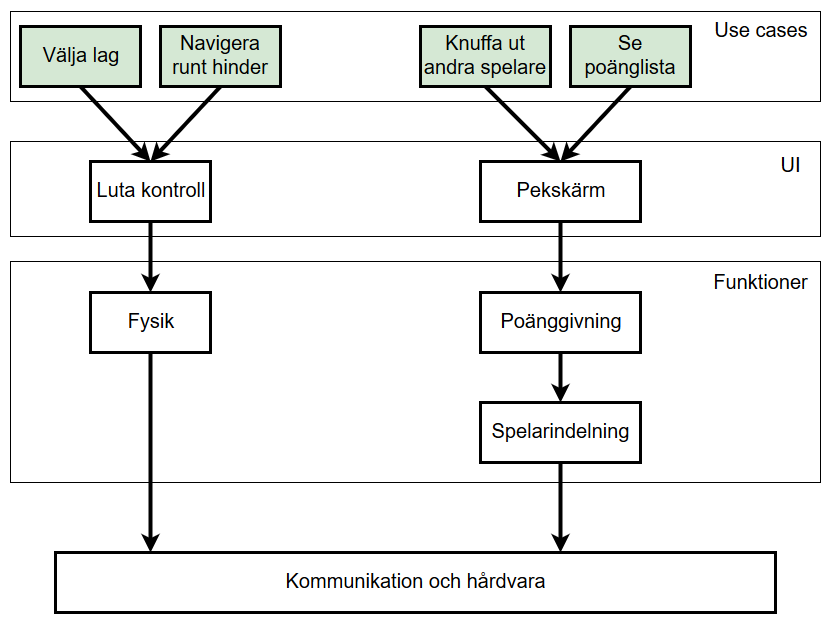
\includegraphics[scale=0.3]{systemanatomi_spel}
    \caption{Överblick av systemanatomin för spelet}
    \label{fig:systemanatomi_spel}
\end{figure}


\pagebreak

\subsection{Moduler}
\label{moduler}
Projektgruppen använde sig av den generella strukturen av systemet, kundens krav och systemanatomin för att skapa en mer detaljerad arkitektur. I figur \ref{fig:konceptarkitektur} kan man se den övergripande strukturen av modulerna som finns i applikationen.

\begin{figure}[h]
    \centering
    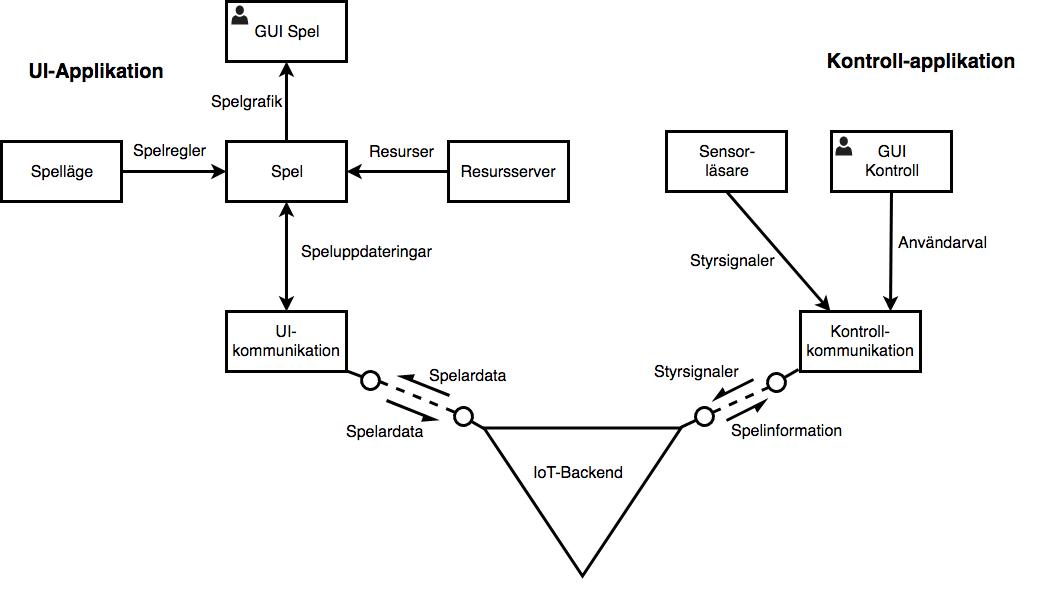
\includegraphics[scale=0.3]{konceptarkitektur}
    \caption{Överblick av systemets moduler}
    \label{fig:konceptarkitektur}
\end{figure}

\pagebreak


\subsubsection*{Ansvarsområden}
Varje modul i systemet har ett eget ansvarsområde. Nedan följer en förtydling på vad varje modul ansvarar för.

\begin{labeling}{\small{\textbf{Kontrollkommunikation}}}
    \item [\small{\textbf{GUI Spel}}]
        \begin{itemize}
            \item Visa upp spelplanen
            \item Visa upp menyer
            \item Starta spel med specifika inställningar
            \newline
        \end{itemize}

    \item [\small{\textbf{Spelläge}}]
        \begin{itemize}
            \item Sätta upp regler för spelet
            \item Avgöra vilka resurser spelet ska innehålla
            \item Avgöra vad som ska ske vid olika tillfällen i spelet
            \newline
        \end{itemize}

    \item [\small{\textbf{Spel}}]
        \begin{itemize}
            \item Hålla koll på de olika spelarna
            \item Tillhandahålla grundläggande spelmekanik
            \newline
        \end{itemize}

    \item [\small{\textbf{Resursserver}}]
        \begin{itemize}
            \item Lagra vilka resurser som finns
            \item Ladda in resurser
            \newline
        \end{itemize}

    \item [\small{\textbf{UI-kommunikation}}]
        \begin{itemize}
            \item Upprätta uppkoppling mot server
            \item Förpacka data för kommunikation
            \newline
        \end{itemize}

    \item [\small{\textbf{Sensorläsare}}]
        \begin{itemize}
            \item Läsa av data från sensor
            \item Abstrahera sensordata till standardiserad form
            \item Konfigurera sensor
            \newline
        \end{itemize}

    \item [\small{\textbf{GUI-kontroll}}]
        \begin{itemize}
            \item Visa menyer för att gå med i spelinstans
            \item Visa spelinformation om det pågående spelet
            \item Tillhandahålla knappar på skärmen
            \newline
        \end{itemize}

    \item [\small{\textbf{Kontrollkommunikation}}]
        \begin{itemize}
            \item Upprätta uppkoppling mot server
            \item Förpacka data för kommunikation
            \newline
        \end{itemize}

    \item [\small{\textbf{IoT-Backend}}]
        \begin{itemize}
            \item Dirigera data mellan olika Kontroll-applikationer och olika instanser av UI-applikationen
            \item Verifiera koder för att gå med i specifika spelinstanser
            \newline
        \end{itemize}
\end{labeling}


\section{Gemensamma erfarenheter}
Denna del tar upp diverse erfarenheter projektgruppen råkat ut för, både innan och under projektets gång.

\subsection{Erfarenheter av systemanatomi}
Systemanatomin som presenterades under \ref{beskrivning-systemanatomi} användes för att ge en enhetlig och helteckande bild över hur det färdiga systemet skulle se ut. Dock var arbetet med att ta fram själva systemanatomin något som tog relativt lång tid, om det vägs mot den nytta gruppen har haft av denna. Den blev mer ett verktyg som kunde användas för att verifiera resterande arkitekturbeskrivningar. Gruppen känner att själva processen att producera anatomin var nyttigare än den resulterande bilden, då det skapade en öppen dialog om systemets helhet.

\subsection{Tidigare erfarenheter}
Alla av projektets medlemmar hade studerat mer än två år på respektive program innan detta projekt startades. På grund av detta hade alla haft möjligheten att medverka i några större projekt och var därför ganska vana vid hur arbetet gick till. Dock var det få som hade erfarenhet med webbutveckling och spelprogrammering, något som hade stort fokus i detta projekt. Detta var dock inget större problem då de mer erfarna kunde hjälpa resten att komma igång.

\subsection{Nya erfarenheter}
Under projektets gång har alla medlemmar fått använda sig av nya verktyg och metoder som de inte haft tidigare erfarenhet av. De projektmedlemmar som tidigare saknade erfarenhet inom webbutveckling och spelprogrammering har fått chansen att sätta sig in i dessa. För att förbättra denna process hjälpte de som redan var erfarna inom ämnet till med att svara på frågor och komma med tips och idéer. Under projektets gång tillkom en del nya paket och ramverk. Ett exempel på detta är PIXI.JS, ramverket UI-applikationen använder för att rita ut spelet. Det var ingen i projektgruppen som hade jobbat med detta ramverk innan, så några i gruppen fick tillsammans sätta sig in i hur det fungerade och utbilda resterande vid behov. Detta gällde även en del av det olika npm-paketen som installerades och användes i projeket.


\subsection{Tidsbrist}
I början av projektet hade gruppen bra tidsplanering och lämnade in första iterationen i god tid för att sedan ta det lugnt. I början av iteration två satsade gruppen i huvudsak på utveckling och lämnade dokumentskrivning till senare, vilket visade sig vara en missbedömning. Detta ledde till att det blev stressigt framåt slutet av iteration två vilket kan ha påverkat dokumentkvaliteten negativt. Gruppen noterade dock detta och tog upp på kommande gruppmöten hur de skulle kunna göra det bättre inför kommande iterationer. Nästa iteration delades upp i en tydligare utvecklingsfas och dokumentfas, vilket tillät en bättre planering och fördelning av tiden.

\subsection{Tekniska erfarenheter}
Projektgruppen utvecklade applikationen i ramverket React som har något som kallas för states. Projektgruppen märkte att det snabbt kunde bli något rörigt när man introducerade flera lager av komponenter. Detta problem löser andra webbapplikationer genom extra verktyg för state-hantering, och gruppen reflekterade över dessa men beslutade emot att använda något liknande. Det visade sig dock i senare delen av projektet att hanteringen av states blev något rörig, då gruppen använt sig av fler komponenter än vad som först uppskattats. Detta ledde till att implementationen av nya komponenter som hamnade mellan redan existerande komponenter blev något jobbig. Detta berodde främst på att data som tidigare skickats från komponent \texttt{A} till \texttt{C} nu behövde skickas från \texttt{A} till \texttt{B} och sen vidare från \texttt{B} till \texttt{C}, när komponenten \texttt{B} introducerades mellan \texttt{A} och \texttt{C}. Detta ledde till att all data som tidigare skickades mellan \texttt{A} och \texttt{C} nu också behövde skickas till \texttt{B}, trots att det kunde vara data \texttt{B} inte använde sig av. En grafisk överblick kan ses i figur \ref{fig:middle_component}

\begin{figure}[H]
    \centering
    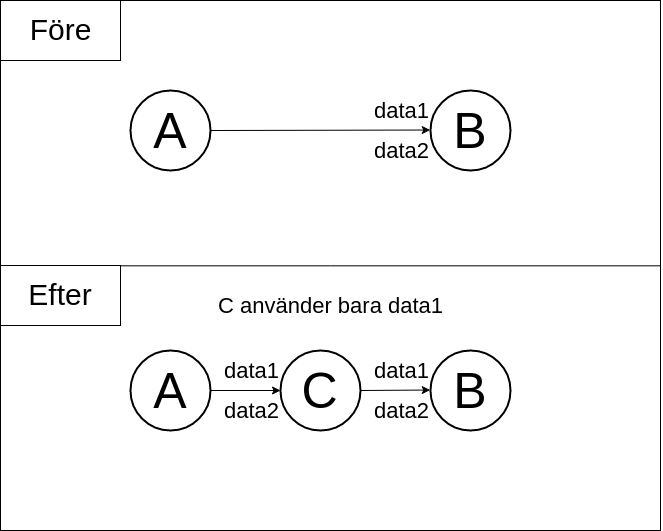
\includegraphics[scale=0.5]{middle_component}
    \caption{Överblick över hur implementation av mittenkomponent kan ge ett ineffektivt dataflöde}
    \label{fig:middle_component}
\end{figure}

\subsection{Erfarenheter med kundkontakt}
Under projekts gång har gruppen haft den stora nyttan av en nära kommunikation med kunden. Tidigt bjöds kunden in i en Slack-kanal med samtliga medlemmar, vilket ledde till en betydligt mer personlig kommunikationen än den som uppnås med mail. Gruppen har också utnyttjat kundens kontor och valt att arbeta där så mycket som möjligt. Då kunden uppmanade till att ställa frågor förtydligades diverse oklarheter snabbt vilket ledde till mer produktivt arbete. Den nära kundkontakten har också lett till en mer öppen dialog kring skapande och verifiering av produktkrav. I projektets början fördes en dialog kring krav tills kravspecifikationen ansågs vara tillräcklig. Under senare delen av projektet har kunden fått flera demonstrationer av produkten för verifiering av att den följer deras krav och vision.



%%%%%%%%%%%%%%%%%%%%%%%%%%%%%%%%%%%%%%%%%%%%%%%%%%%%%%%%%%%%%%%%%%%%%%
%%% lorem.tex ends here

%%% Local Variables:
%%% mode: latex
%%% TeX-master: "demothesis"
%%% End:

\chapter{Diskussion}
\label{cha:discussion}

I följande del presenteras olika tankar och idéer som uppkommit baserat på denna rapports innehåll och det genomförda projektet. De resultat som har uppnåtts väcker flera intressanta tankar och frågor. Det finns möjliga förbättringar till metoden som i efterhand har uppdagats. Arbetet existerar även i en samhällelig och etisk kontext som bör lyftas.

\section{Resultat}
\label{sec:discussion-results}

%Fanns alternativa implementationssätt?
Det fanns i det genomförda projektet många val som kunde leda till annorlunda resultat. Många teknikval har behövt tas för att färdigställa produkten. En stor andel av dessa har tagits enligt önskemål från kunden och det är inte troligt att kundens värde skulle kunna öka om dessa inte följdes. I denna kategori faller användning av React samt att koden skrevs i ren Javascript.

Många av de tekniska val som gruppen har tagit relaterar till speldelen av produkten. Ett stort sådant var att skapa spelet som ett mer allmänt ramverk för olika spellägen istället för ett specifikt spel. Det är troligt att projektet hade förändrats mycket om det andra alternativet hade valts. Då ett av kundens viktigaste önskemål var att enkelt kunna vidareutveckla projektet bedömdes dock det mer generella valet ge mer värde. Val av bibliotek för spelet var också ett viktigt avgörande i projektet. Flera alternativ diskuterades som till olika grad förlitade sig på färdiga paket för fysik, grafik och logik. Den slutgiltiga lösningen med PixiJS har givit stora möjligheter att skapa det system som önskades och gav även mycket stöd i rendering av spelets grafik. Utan färdiga bibliotek hade arbetet troligen tagit alldeles för lång tid. Användning av många stora bibliotek kan istället introducera oönskade begränsningar på projektets struktur.

%Vad återstår för att kunden skall få ut fullt värde av produkten?
Den slutgiltiga produkten innehåller några enkla spellägen som fungerar till fullo. Dessa kräver ingen vidareutveckling från kundens sida utan kan användas som tilltänkt efter leverans. Det är dock troligt att kunden vill introducera fler spellägen. En viss del av produktens värde ligger i hur hög utökningsbarhet som har uppnåtts för att underlätta denna process. Utförlig dokumentation har även skapats för att minimera tiden som krävs för att sätta sig in i systemet. Med detta är förhoppningen att skapandet av nya spellägen ska gå mycket smidigt och inte kräva förståelse för implementationsdetaljer.

%Lyckades ni förbättra/fortsätt något från tidigare projekt?

%Viktigaste lärdomar inför framtiden.

% Övrig mumbo-jumbo :S
Det fanns genom projektet en viss förvirring och osäkerhet gällande arbetet med systemanatomin. Ofta fanns stora skillnader i olika medlemmars uppfattning av hur anatomin skulle vara konstruerad. Det är möjligt att en otillräcklig förståelse för konceptet kan ha lett till att den framtagna modellen tappat mycket värde. Det är möjligt att svaret på frågeställning \ref{fs:fs_3} kunde haft ett större värde om det fanns fler ingående erfarenheter av arbete med systemanatomier. Gruppen diskuterade även huruvida relevansen av detta dokument kan förändras mycket mellan olika typer av projekt och utvecklingsmetodik. Det genomförda projektet befinner sig på en hög abstraktionsnivå med liten hårdvarukoppling. Det är av intresse hur systemanatomins nytta skulle se ut i mer hårdvarunära projekt, men detta har inte undersökts vidare.

Det är mycket troligt att resultat av projekterfarenheter har påverkats av att denna studie av processen har pågått parallellt. Gruppmedlemmarna har haft en medvetenhet om att projektet ligger till grund för detta arbete och även tagit del av seminarier som skapat en djupare reflektion. Detta delade fokus har troligen påverkat projektets utveckling. Det är dock troligt att utförandet av denna undersökningen parallellt är nödvändigt för att ge en tillräcklig insikt i projektet. Även om gruppens erfarenheter är att projektet ej kan anses till fullo representera typisk mjukvaruutveckling bedöms detta inte påverka resultaten i alltför stor utsträckning.

Testningen som gjorts under projektets gång har lämnat en lite önskande efter mer. De flesta test har utförts direkt efter koden som testats skrivits, och utav samma person och därmed inte varit en så utarbetad process man hade kunnat önskat. Detta berodde till stor del på avsaknad av ordentlig struktur från början och okunnighet från gruppens sida då få gruppmedlemmar var vana användare utav automatisk testning.

 En bit in i projektet började testningen komma ifatt och ett antal automatiska tester började formas. Möjligtvis blev testerna inte optimala då tidigare erfarenheter utav testning var bristande. En lärdom dras av detta att påbörja testningen i ett tidigare skede för att verkligen komma igång med det, kanske till och med testdriven utveckling \cite{TDD} vore ett bra alternativ. Om man formar produkten efter testerna blir man tvungen att skriva tester och får som en slags checklista att bocka av när testerna klarar sig. Dock hade det inte fungerat med vår nuvvarande setup då vi har en regel som säger att man inte kan synka med versionhanteringssystemet om test inte går igenom. 

Manuella tester är det som använts flitigast under projektets gång då manuella tester går snabbt och gruppen vet väl sedan tidigare hur de ska genomföras. De flesta har skett inofficiellt utav samma testare vilket kan vara en nackdel men utvecklingen har ändå gått framåt i en bra hastighet. Det finns ett par officiella tester \ref{fig:manual_test} som gjorts för att kolla så produkten lever upp till vad som är utlovat i kravspecifikationen. Dessa har gjorts utav en testare i samband med testledaren för att säkerställa att allting gått rätt till.

Då det ej fanns mycket utav tidigare kompetens inom testning skapade gruppen lite olika tester för att lära sig använda verktyget. Mycket upplärning skedde i början för att veta hur tester definieras och vad de gör. Det skapades olika sorters testning i syfte för att få bredare kunskap och få lärdom över vad de olika testerna faktiskt gjorde. Det användes allt från assertion testing\cite{assertion-testing} till snapshot testing\cite{snapshot-testing}.

Resultatet från den utförda enkätundersökningen uppnåde till stor del de önskade resultaten. Målet av undersökningen var att få ett snitt betyg över sex. Detta uppfylldes på alla frågor utom en, "Jag tycker det var svårt att förstå spelets regler", som fick betyget 5.8. Från att åtgärda detta problem implementerade gruppen en inforuta på både kontrollern och UI:t. Inforutan beskriver reglerna för spelläget som spelas. Enkätundersökningen utfördes inte ytterigare en gång efter inforutan hade implementerats. Detta hade varit intressant för att undersöka inforutans effekt på betyget. När medianen undersökts för de övriga resultaten syns det att detta resultatet är högre än medelvärdet. Detta tyder på att det var en större andel som röstade högt än lågt, men att de som röstade lågt, satte väldigt låga poäng.

% Are there anything in the results that stand out and need be
% analyzed and commented on? How do the results relate to the
% material covered in the theory chapter? What does the theory
% imply about the meaning of the results? For example, what
% does it mean that a certain system got a certain numeric value
% in a usability evaluation; how good or bad is it? Is there
% something in the results that is unexpected based on the
% literature review, or is everything as one would theoretically
% expect?

\section{Metod}
\label{sec:discussion-method}
%Vilka konsekvenser fick de valda metoderna för resultaten?
Den rolluppdelning som har gjorts har troligen påverkat delar av projektet och därmed resultatet. Rollerna har fört med sig dokumentationsbeslut och arbetsprocesser. Vissa ansvarsområden överlappar delvis och det är tänkbart att andra resultat hade nåtts om dessa hade slagits ihop till färre roller. Det finns även specifika roller som inte använts. Exempel på detta är tekniska experter över vissa områden i projektet. Denna sorts roll har i det utförda projektet till viss del uppstått spontant genom personer som är mer insatta i viss teknik. Det är möjligt att resultaten hade sett annorlunda ut om denna uppdelning hade skett i förtid och mer explicit.

%Fanns det alternativ?
Ett alternativ till den iterativa, agila arbetsmetodiken i projektet hade varit en mer traditionell vattenfallsmodell. Detta går dock mot gruppmedlemmarnas tidigare erfarenheter av problem med denna sorts arbetsprocess. Det skulle även finnas organisatoriska problem med detta utifrån planeringen av den kurs projektet ingår i. Denna jämförelse undersöks vidare i individuell rapport \ref{individual:lieth-wahid}. Även inom iterativa arbetsmetoder finns det olika alternativ som har övervägts. Istället för att basera arbetsmetodiken på Scrum skulle exempelvis Kanban\cite{kanban} eller Rational Unified Process\cite{RUP} kunnat användas.

Inom den variant av Scrum som har använts genom projektet finns många valmöjligheter som har förändrat utvecklingsprocessen. Längden på sprints, tid avsatt för vissa möten och uppdelning av arbetsuppgifter är saker som troligen har påverkat arbetet märkbart. Vilka delar av Scrum som har tagits med i projektets utförande har troligen också påverkat mycket. Exkludering av stand-up meetings är ett sådant centralt beslut. I det fallet ansågs det inte effektivt logistiskt. Här hade andra alternativ till daglig kommunikation kunnat övervägts för att uppnå samma effekter.

Arbetet med enkäterna och demonstrationerna påverkade troligen resultatet på helt olika sätt. Enkätundersökningen gjordes under projektets senare skede, under en tid då utvecklingsarbetets fokus var på kvalitet och inte funktioner. Alltså var det svårt för gruppen att använda sig av resultatet från denna undersökning på ett sätt som faktiskt visades i produkten. En möjlig förbättring på denna metod skulle vara att hålla flera enkätundersökningar under projektets gång och i sin tur använda sig av feedbacken i utvecklingsarbetet. Nu användes istället resultatet för att verifiera kvaliteten av en nästan färdigställd produkt. Detta skilde sig dock med demonstrationerna för kund. Denna feedback kom kontinuerligt under utvecklingsfaserna och feedbacken ledde till direkta ändringar av utvecklingen. En eventuell förbättring till denna metoden är att mer formellt dokumentera den feedback som gruppen får, för att senare verifiera dess påverkan på produkten.

%Källkritik.
En del av de använda källorna kommer från dokumentation över produkter skapade av företag. Här finns anledning att tro att ett visst intresse finns för att presentera dessa produkter med viss positiv vinkling. Dock har dessa källor endast används för tekniska specifikationer och i detta anses inte någon möjlig vinkling påverka korrektheten.

% This is where the applied method is discussed and criticized.
% Taking a self-critical stance to the method used is an
% important part of the scientific approach.
%
% A study is rarely perfect. There are almost always things one
% could have done differently if the study could be repeated or
% with extra resources. Go through the most important
% limitations with your method and discuss potential
% consequences for the results. Connect back to the method
% theory presented in the theory chapter. Refer explicitly to
% relevant sources.
%
% The discussion shall also demonstrate an awareness of methodological
% concepts such as replicability, reliability, and validity. The concept
% of replicability has already been discussed in the Method chapter
% (\ref{cha:method}). Reliability is a term for whether one can expect
% to get the same results if a study is repeated with the same method. A
% study with a high degree of reliability has a large probability of
% leading to similar results if repeated. The concept of validity is,
% somewhat simplified, concerned with whether a performed measurement
% actually measures what one thinks is being measured. A study with a
% high degree of validity thus has a high level of credibility. A
% discussion of these concepts must be transferred to the actual context
% of the study.
%
% The method discussion shall also contain a paragraph of
% source criticism. This is where the authors’ point of view on
% the use and selection of sources is described.
%
% In certain contexts it may be the case that the most relevant
% information for the study is not to be found in scientific
% literature but rather with individual software developers and
% open source projects. It must then be clearly stated that
% efforts have been made to gain access to this information,
% e.g. by direct communication with developers and/or through
% discussion forums, etc. Efforts must also be made to indicate
% the lack of relevant research literature. The precise manner
% of such investigations must be clearly specified in a method
% section. The paragraph on source criticism must critically
% discuss these approaches.
%
% Usually however, there are always relevant related research.
% If not about the actual research questions, there is certainly
% important information about the domain under study.

\section{Samhälleliga och etiska aspekter}
\label{sec:work-wider-context}

Projektet som har utvecklats har helt publicerats som open-source under licensen MIT\cite{MIT-license}. Detta är en mycket öppen licens som tillåter fri användning av programvaran för de flesta syften. Genom att dela med sig av all kod kan andra utvecklare välja att använda delar av den producerade koden i egna projekt eller lära sig av de designbeslut som tagits. Denna spridning av information och erfarenheter gör att mängden resurser för liknande framtida projekt ökar. Eftersom projektet är helt öppet och inte dolt bakom någon betaltjänst eller liknande hinder erbjuds alla samma möjlighet att ta del av det.

Projektet som har genomförts har från kundens sida syftet att demonstrera ett system för Internet of Things. Detta gör att projektet till viss del kan anses marknadsföra IoT som koncept. Direkta effekter av den utvecklade produkten på samhälle och miljö anses mycket små. Istället läggs här ett större fokus på indirekt påverkan från den mer uppkopplade värld som slutprodukten bidrar till att demonstrera.

%Samhälleliga
\subsection{Samhälle}
Introduktionen av IoT-koncept innebär stora förändringar av samhället. På en stor skala kan bussar och bilar tänkas vara uppkopplade mot servrar som kan erbjuda många logistiska optimeringsmöjligheter. Även i andra viktiga samhällsinstanser som sjukvård och räddningstjänst kan en mer uppkopplad värld erbjuda många möjligheter. På en mindre skala påverkar IoT varje enskild person och interaktionen mellan människor. Allt fler av objekten i vårt hem kopplas mot internet. Detta påverkar hur vi använder dessa och därmed våra levnadsmönster.

%Miljö
\subsection{Miljö}
Då fler och fler saker kopplas upp mot internet skapas nya behov av nätverk. Både i de uppkopplade apparaterna och i den kringliggande infrastrukturen krävs hårdvara som klarar av större mängder nätverkstrafik. Detta introducerar en ökad energianvändning på flera nivåer i nätverksstrukturen. Små objekt som tidigare innehållit ingen eller endast väldigt enkel elektronik behöver kunna upprätthålla nätverkskommunikation. Även behandling av de stora mängder data som kan skapas är en stor del av IoT-konceptet. Servrar som under lång tid utför tunga dataanalyser kräver stora mängder energi för att utföra sina uppgifter.

IoT erbjuder även många möjligheter för miljöarbete. Insamling av data genom många små sensorer och behandling av denna kan tänkas möjliggöra övervakning av processer som påverkar miljön. IoT tillåter också effektivisering av många industrier, vilket kan tänkas leda till en mer hållbar utveckling. Exempel på en industri med stor miljöpåverkan och möjligheter inom IoT är jordbruk. Här kan olika uppkopplade lösningar optimera resursanvändning och effektivisera processer, vilket ger en positiv miljöpåverkan.\cite{IoT-agriculture}

%Etiska
\subsection{Etik}
Med många små uppkopplade moduler skapas stora mängder data. Denna data har ofta en obetydlig natur i sig självt, men kan få värde i kombination med annan. I de fall denna data beskriver egenskaper hos personer eller deras aktiviteter introducerar detta flera etiska dilemman. Det blir aktuellt att ställa frågor om vem som äger datan och vad den får användas till. Många IoT-lösningar erbjuds som tjänster där all data lagras och hanteras på företags servrar. Det är då förståeligt att användare känner en viss oro för hur den används och sprids. Här läggs ett stort ansvar på företag och organisationer att ta fram riktlinjer för hur man behandlar denna data.

% There must be a section discussing ethical and societal
% aspects related to the work. This is important for the authors
% to demonstrate a professional maturity and also for achieving
% the education goals. If the work, for some reason, completely
% lacks a connection to ethical or societal aspects this must be
% explicitly stated and justified in the section Delimitations in
% the introduction chapter.
%
% In the discussion chapter, one must explicitly refer to sources
% relevant to the discussion.

\chapter{Slutsatser}
\label{cha:slutsatser}

Baserat på de uppnådda resultaten kan frågeställningarna svaras på i stor utsträckning. Det genomförda projektet kan därmed erbjuda vissa intressanta insikter enligt syftet med denna rapport. I följande stycken presenteras de slutsatser som har uppnåtts och arbetets vidare lärdomar.

\section{Frågeställningar}

\subsection*{\ref{fs:fs_1} Hur kan ett realtidsspel som använder sig av Cybercoms backend implementeras så att man skapar värde för kunden?}

Ett system baserat runt Cybercoms backend har implementerats. Systemet består av ett spel med flera olika spellägen. Speciellt arbete har lagts på att försäkra sig om att spelet känns responsivt för användarna. Detta ger kunden värde då det demonstrerar effektiviteten i den existerande backenden.
Med möjligheten att skapa nya spellägen finns stor potential till vidareutveckling av produkten. Detta ger kunden stort värde för framtida användning av systemet.

\subsection*{\ref{fs:fs_2} Vilka erfarenheter kan dokumenteras från programvaruprojektet som kan vara intressanta för framtida projekt?}

En organisatorisk erfarenhet som kan tas med från projektet är hur mjukvaruutveckling och dokumentskrivning kan balanseras. Att arbeta mer kontinuerligt och parallellt med dokument och kod i projekt har visat sig fördelaktigt. På den tekniska sidan finns flera erfarenheter av React-utveckling. En stor sådan är vikten av att organisera lager av komponenter. React har visat sig lätt introducera problem med rörig kod då inga verktyg för state-hantering används.

\subsection*{\ref{fs:fs_3} Vilket stöd kan man få genom att skapa och följa upp en systemanatomi?}

En systemanatomi kan erbjuda viss hjälp med att ge en översiktlig bild över ett system. I en grupp kan den även bidra till en mer gemensam bild av vad som ska skapas och därmed förhindra missförstånd. Att ta fram systemanatomin har dock visat sig vara en svår process. I det utförda projektet upplevdes det svårt att få en gemensam bild över vad systemanatomin representerar. Det är troligt att detta har reducerat det stöd som gruppen har fått av modellen.

\subsection*{\ref{fs:fs_4} Hur kan kontinuerliga användardemonstrationer användas i utvecklingsfasen för att förbättra ett spels kvalitet?}

I det utförda projektet har spelet flera gånger demonstrerats för kunden. Dessa demonstrationer har använts som kontroller över att utvecklingen går i rätt riktning. De har även varit möjligheter för kunden att förtydliga eller justera sina mål med projektet. Idéer till olika lösningar har också kunnat diskuterats öppet.

\section{Måluppfyllelse}

Det genomförda projektet har till stor del lyckats skapa värde för kunden. Det slutgiltiga systemet demonstrerar flera kvalitetsaspekter hos kundens IoT-backend. Spelet erbjuder också goda möjligheter till vidareutveckling genom nya spellägen. Slutprodukten anses därför väsentligen ha uppfyllt de mål som projektet utgått från.

Denna rapport ger en god bild över den utvecklingsprocess som har följts och resultaten från utvecklingsarbetet. Genom erfarenheter och reflektioner från det utförda projektet har de presenterade frågeställningarna kunnat svarats på. Med avseende på projektets storlek anses dessa slutsatser vara av god relevans. För ytterligare generella aspekter av frågeställningarna skulle troligen flera olika projekt behöva studeras, men detta ligger utanför detta arbete.

\section{Viktiga insikter}

Från detta arbete finns flera intressanta insikter om både teknisk implementation och utvecklingsprocessen. Det utförda projektet presenterar en möjlig variant av agil utveckling som kan ge en värdefull slutprodukt. Detta visar att en mer avskalad variant av ett utvecklingsramverk som Scrum kan passa bra för projekt av mindre skala.

Många dokument har producerats i projektet och skapat stöd för gruppmedlemmarna. Dessa dokument har på olika sätt kommit till nytta innan, under och efter utvecklingsarbetet. Värdet hos olika sorters dokument är en nyttig insikt från det utförda projektet. Speciellt har det reflekterats över användning av systemanatomier. Denna typ av dokument, som till viss del skiljer sig från många andra systemmodeller, kan vara ett nyttigt verktyg att ta med sig till framtida projekt.

% This chapter contains a summarization of the purpose and the research
% questions. To what extent has the aim been achieved, and what are the
% answers to the research questions?
%
% The consequences for the target audience (and possibly for researchers
% and practitioners) must also be described. There should be a section
% on future work where ideas for continued work are described. If the
% conclusion chapter contains such a section, the ideas described
% therein must be concrete and well thought through.

\appendix
\chapter{Deepstream serialisering och rundturstid av Tim Håkansson}

\section{Introduktion}

Under de senaste åren så har allt fler och fler enheter blivit inkopplade i IoT ekosystemet och än så länge ser det ut att fortsätta frammåt med hela 24 miljarder förväntade enheter uppkopplade\cite{IoT-ecosystem}. För att realisera denna utvecklingen behövs det robusta lösningar som klarar av att hantera, lagra och slussa data i realtid, samtidigt som lösningen behöver vara enormt skalbart. Det är här tjänsten deepstream\cite{deepstream} kommer in i bilden. Tjänsten annonserar sig att vara en snabb, enkel och säker tjänst som sedan 2015 börjat komma upp lite här och där. Deepstream används i ett flertal olika tjänster, med de mest noterbara briteback och ticketmaster\cite{ds-usecases}.

Projektet, som pappret utgår ifrån, utfördes under vårterminen 2018 och använde sig utav deepstream för att skicka, ta emot och hantera data. Anledningen till just deepstream var att våran kund, Cybercom, använde sig av denna tjänsten under sin utveckling av IoT lösningar. Eftersom deepstream annonserar sig att vara en kraftfull server som klarar av att hantera data mellan olika enheter i realtid, så finns det en motivering att undersöka hur väl det anpassar sig in i spelvärlden, där responsivitet för indata är a och o.

\subsection{Syfte}
\label{subsec:tim-aim}
Projektet som har utförts bygger en hel del på att nätverkslösningen som implementerats är snabb och skalbar för att uppnå maximal responsivitet för många användare. För att uppnå detta krävs en djupare förståelse för hur deepstream hanterar data beroende på olika inverkningar i systemet. Inverkningarna som tas upp i detta pappret är belastning, datastorlek och hur biblioteket används (gällande RPC gentemot event).

Genom att då undersöka dessa förhållanden kan teamet ta lärdom av hur data ska hanteras och när och hur data ska skickas.

\subsection{Frågeställning}
\label{subsec:tim-research-questions}
För att göra denna undersökninen krävs några fundementala frågor som behöver besvaras, dessa presenteras nedan:

\begin{enumerate}
\item Hur påverkas responsiviteten i nätverket beroende på datastorleken?  

\item Under vilka förhållanden är det bättre att använda RPC över event och vise versa?

\item Lämpar det sig att använda sig av deepstream för att hantera indata i ett realtidsspel?

\end{enumerate}
\subsection{Avgränsingar}
\label{subsec:tim-delimitations}
Då det inte går att deligera hur mycket tid och resurser som helst på undersökningen behöver vissa avgränsningar göras. Till en början så undersöks inte deepstream i en verklig miljö, dvs undersökningen görs på ett lokalt nätverk. Detta leder till att responstiderna till stor del inte reflektera rundturstiden (RTT) för nätverket då all data skickas på ett lokalt nätverk.

Dessutom så kommer inte responstiderna ta skalbarheten in i beräkningen då resurser för att koppla upp ett stort antal användare inte finns tillgängligt. Så responstiderna är endast med avseende på ett tomt nätverk och därmed handlar det mer om hur snabbt deepstream kan arbeta med datan innan den skicka datan vidare.

I pappret hanteras inte heller deepstreams records då denna strukturen inte är relevant för projektet.

\section{Bakgrund}
\label{sec:tim-background}
När det gäller datakomprimering så finns det andra studier som har gjorts som analyserat serialisering och deserialisering för olika typer av datastrukturer. I ''Performance Evaluation of Object Serialization Libraries inXML, JSON and Binary formats'' skriven av Kazuaki studerades olika data format, JSON, XML och binära format och hur dessa förhåller sig till varandra. Detta gäller datastorlek och hastighet för serialisering och deserialisering. Utöver det så granskas även olika bibliotek för samma format, där alla körs i Java. Detta för att få en bredare syn på hur formatet påverka exekveringstiden och inte hur väloptimerat biblioteket är. Resultatet från studien visar att binär data generellt sätt är snabbare och mer komprimerat i alla fall.

\section{Teori}

\label{sec:tim-theory}
För att göra undersökningen behövs en viss grund av begrepp och teminologier fastställas för att underlätta arbetet i senare skedde.

\subsection{JSON}
JSON\cite{json} är ett dataformat för att lätt kunna hantera data, både för en dator och en användare. Formattet bygger översiktligt på fält med värden, objekt med flera fält och listor med objekt. Men listor kan även finnas i objekt och listor kan också innehålla fält. Formatteringen kan se ut som i figur \ref{fig:jsonformat} där det finns ett objekt med en lista av anställda.

\lstset{language=Java}
\begin{figure}[h]
  \begin{minipage}[c]{5cm}
    \begin{lstlisting}
{
    "name": "John",
    "age": 30,
    "cars": {
        "car1": "Ford",
        "car2": "BMW",
        "car3": "Fiat"
    }
} 
    \end{lstlisting}
  \caption{JSON formattering}
  \label{fig:tim-jsonformat}
  \end{minipage}
\end{figure}

\subsection{Deepstream}
\label{subsec:tim-deepstream}
Deepstream är en Javascript-baserad tjänst med skalbarhet och datahantering i realtid i åtanke. Saker som utmärker detta gränssnitt är dess realtidsdatabaser, autentisering och behöver ingen backend utveckling för att fungera. För att få en fungerande backend behöver man endast starta en deepstream server och sedan är allt igång. Resten av integreringen sker på klientsidan av applikationen, så all datahantering sker utan någon form av serverprogrammering. För att få denna moduläriteten hanteras all data av servern med hjälp av tre enkla koncept. Dessa koncept är records, events och RPCs (Remove Procedure Call) och beskrivs mer ingående nedan. 

\subsubsection{Deepstream record}
Idén med records är att kunna lagra, updatera och ta bort data utan att denna datan försvinner efter körning. Detta samtidigt som att datan ska vara synkroniserad mellan alla uppkopplade enheter. För att uppnå detta använder deepstream en databas server som kan konfigueras till att hantera Postgres, MongoDB, ElasticSearch eller RethinkDB. 

Då detta pappret inte kommer hantera records så kommer ingen mer ingående förklaring ges\cite{ds-storingdata}.

\subsubsection{Deepstream event}
Ett event (även kallad kanal) kan ses som en direkt länk mellan flera publicerare och prenumeranter. En publicerare är helt enkelt en användare som skickar data till deepstream server via en viss kanal som ges av en sträng (vanligtvis med format ''projekt/kanalnamn''). När deepstream servern mottagit datan skickas den vidare till alla användare som prenumerera på samma kanal. 

Datan som skickas är i JSON-format och kommer inte lagras på deepstream servern. Därmed är tanken med events att det ska vara snabbt och enkelt att skicka data. 

\subsubsection{Deepstream RPC}
Utifrån events och records behövs det något enkelt sätt att skicka data samt få ett svar på den skickade datan. Detta kan vara ett enkelt fall då man implementera en addition RPC på en client och anropa den från en annan för att få ett svar på beräkningen. Detta är ett av de mest triviala exemplet, men all form av validering, beräkning eller liknande som man vill göra på en annan klient görs enklast med hjälp utav RPCs.

På samma sätt som i events så skickas datan i ett JSON-format, både för anropp och svaret från RPCn.

\subsection{Rundturstid}
När rundturstid nämns i denna delen av pappret menas tiden det tar att skicka en förfrågan till en annan klient i nätverket och få tillbaka ett svar. Det vill säga tiden det tar att skicka ett meddelande till deepstream servern, få servern att skicka vidare till en annan klient som sedan skicka tillbaka ett svar genom servern. Det betyder \textbf{inte} tiden det tar att få ett direkt svar från deepstream servern då detta inte ger ett relevant värde eftersom att klienter aldrig kommunicera direkt med servern.

\subsection{Wireshark}
Wireshark är ett verktyg för att analysera nätverkstrafik för att se över vad som skickas, över vilket protokol och vem som skicka eller tar emot datan. Detta ger användaren en bra förståelse för hur olika protokol fungera på en lägre nivå.

\subsubsection{Interface}
Utifrån det kan man ställa in vilket interface\cite[p.~364]{networking} man lyssnar på, detta inkluderar generellt bluetooth, ethernet och loopback. I detta pappret kommer loopback interface användas, detta interface är till för att skicka nätverksdata till och från samma dator. Det vill säga den data som inte skickas till en annan dator.

\section{Metod}
\label{sec:tim-method}

För att uppnå ett relevant resultat sattes enklare simulationer upp på olika de olika gränssnitten. Detta gjordes genom att sätta upp en server på en dator som klarar av mer belasning och sedan ansluta flera olika instanser av clienter på några olika datorer. Genom att köra på några olika datorer minskar risken att clienterna kommer vara flaskhalsen i systemet.

\section{Resultat}
\label{sec:tim-results}
Efter att ha följt metoderna från avsnitt \ref{sec:tim-method} beskrivs resultaten för de olika undersökningarna nedan. 

\subsection{Serialisering}
När endast ett objekt skickades kunde man observera att datan som skickades över event såg ut som i figur \ref{fig:tim-eventdata1} som illustrerar en hexdump från Wiresharks applikationslager. Här är den relevanta datan på rad \textit{0020} med start på \textit{\{}. Hexdumparna för RPC och event samt 1-5 objekt finns tillgängliga i appendix \ref{app:hexdumps}. Vad man kan se från resultatet är att deepstream inte gör någon form av komprimering av JSON-objekt för att minimera datan som skickas över nätverket. Dock så tar den bort alla former av blanksteg och tabbar, då dessa inte har någon påverkan på slutresultatet av ett JSON-Objekt. Från att kolla på datan ser vi att deepstream även skickar med lite extra data för att hålla koll på vad för anropp som görs. Det går även att se att antalet bytes som skickas för JSON-objektet är 74 bytes per objekt med 1 byte som kommatecken till att separera alla JSON-objekt. Detta går att läsa av i de olika hexdumparna från appendix \ref{app:hexdumps}. Denna anmärkningen används för resultatdelen av avsnitt \ref{subsec:tim-result-response}.

\subsection{Rundturstid}
\label{subsec:tim-result-response}
Resultatet av rundturstiden från metoden som beskrevs i avsnitt \ref{subsec:tim-method-response} presenteras i figur \ref{fig:tim-response-graph}. Från denna kan det ses att rundturstiden beror linjärt på hur mycket data som skickas. Vad som är intressant är att en RPC är mycket snabbare med att skicka data när det gäller att få ett svar tillbaka, samtidigt som att responstiden varierar mycket mindre. Det går dock inte att se någon speciell skillnad på komplexiteten hos båda då rundturstiderna ser ut att öka med samma hastighet. Notera att skalan är i millisekunder och att skillnaden mellan båda endast är ca 4 ms. I fallet då 990 JSON-objekt skickas det $74*990+989=74249$ bytes med data, vilket är ett extremfall som troligtviss aldrig händer i verkligheten.

\begin{figure}[t]
    \center
    \begin{tikzpicture}
        \begin{axis}[
            xlabel={Antal JSON-objekt},
            ylabel={Medeltid från 100 anropp (ms)},
            ytick={0,2,...,10},
            xtick={0,33,...,99},
            xticklabels={0,330,...,990},
            legend pos=north west,
            ymin=0,
            ymax=10,
            grid style=dashed,
            domain=0:100,
        ]
        \addplot[color=red,]
            table[x expr=\coordindex+1, y index=0]{individuall/tim/data/event_avg.dat};
            \addlegendentry{Event}
        \addplot[color=blue,]
            table[x expr=\coordindex+1, y index=0]{individuall/tim/data/rpc_avg.dat};
            \addlegendentry{RPC}
        \end{axis}
    \end{tikzpicture}
    \caption{Responstiden i jämförelse med antal objekt som skickas.}
    \label{fig:tim-response-graph}
\end{figure}

\section{Diskussion}
\label{sec:tim-discussion}
Under arbetets gång har flera olika resultat uppstått, vilket ger en bra bild av hur storleken på datan över deepstream påverkar tiden det tar att skicka den. För att få en bättre förståelse av resultaten så diskuteras resultat, metod och hur metoden har påverkat resultatet nedan. 

\subsection{Resultat}
\label{subsec:tim-discussion-results}
Från undersökningen har två olika resultat beskrivits där den ena handlar om hur deepstream komprimera data och den andra hur deepstream skalas beroende på datastorleken.

\subsubsection{Serialisering}
När det gäller serialiseringen så gör deepstream inga direkta förbättringar för att minska datastorleken, detta beror troligtvis på att Javascript till stor del bygger på JSON-objekt och i och med det finns det en motivering av att fortsätta arbeta med just det formatet. Då behöver inte mycket göras för att omvandla klasser, datastrukturer eller liknande eftersom allt till stor del bygger på JSON och listor.

Frågan är då om deepstream hade tagit nytta av att göra om datan till ett binärt format, vilket enligt avsnitt \ref{sec:tim-background} skulle ge ett bättre resultat. Problemet här är att den binära serialiseringen bygger på att datastrukturen är upplagd på ett visst sätt, och i fallet med Javascript och Protobuf behövs ett helt nytt objekt med setters användas för att skicka datan. Detta kan då leda till att binärdatan får mer overhead för att ens börja serialiseras. Vilket kan visa sig ta längre tid än JSON-objekt, detta skulle dock behövas undersökas vidare för att få ett mer konkret resultat kring serialiseringshastigheter.

\subsubsection{Rundturstid}
Från resultatet kunde man se att RPC är snabbare än att använda sig av event när det gäller att skicka och ta emot data. Anledningen till detta kan ligga i att ett event måste kolla upp vilka användare som prenumerera på en viss kanal två gånger. RPCs behöver endast göra detta en gång då den inte behöver leta upp vem som frågade efter RPCn eftersom denna skickas med i anropet. Utöver det så kan det tillkomma en hel del overhead med events då flera kan lyssna på samma kanal och mer beräkningar behövs då göras, vilket i sin tur kan ge upphov till att spridningen för events är större än för RPCs. Hur RPCs och events är implementerade kan ses i källkoden för deepstream på GitHub\footnote{\url{https://github.com/deepstreamIO/deepstream.io} \newline commit: 98a2f53b0f7ca984a0f0f2f5a89c225c21467687}. 

\subsection{Metod}
\label{subsec:tim-discussion-method}
Metoden som har använts har givit en bättre insyn om hur de olika funktionerna RPC och event fungera i en djupare nivå, samt om deepstream gör någon form av komprimering av data. För komprimering och analysen i Wireshark, så speglar metoden exakt på hur datan serialiseras då detta varken beror på CPU-hastighet, nätverk eller andra oförutsägbara parametrar. Så det går direkt att säga deepstream inte använder sig av någon form av komprimering.

Om man dock blickar bort mot responstiden så finns det mycket som kan påverka resultatet, till en början spelar datorns processor roll, då en snabbare processor ger bättre värden. Dock så borde detta inte reflektera över att RPC är snabbare än event då detta borde dra ner responstiden lika mycket. Andra saker som spelar större roll är hur Javascripten exekveras, i termer av hur datastrukturer hanteras på olika processorer. Detta kan ge större påverkningar på resultatet eftersom sättet Javascript hanterade datastrukturen på datorn som användes för undersökningen kanske fungerade bättre för RPC än för event och därav gav de resulterande resultaten. Detta är något som borde undersökas vidare mellan olika datorer. 

En annan sak som inte reflekteras i resultatet från metoden är att undersökningen endast kördes från och till en lokal dator, så en responstid på < 10 millisekunder är inget man kommer se i verkligheten. Detta eftersom att tiden det tar att skicka datan över ett nätverk inte är inräknat, vilket leder till att det ser ut som att RPCs har ett stort övertag över events. Men om tiden det tar att skicka data från en punkt till en annan ökar, borde inte skillnaden mellan RPCs och events påverkas, då tiden endast reflekterar serialisering, deserialisering och loopbacktiden i datorn (som kan göra andra former av optimeringar då datan inte skickas över ett nätverk).

\section{Slutsatser}
\label{sec:tim-conclusion}
Här sammanfattas resultaten och diskussionen i formen av att svara på frågeställningarna från avsnitt \ref{subsec:tim-research-questions}.

\subsection*{\ref{tim-fs:1} Hur serialisera deepstream datan som skickas över nätverket?}
Som nämnt tidigare görs ingen direkt komprimering av data när man använder sig av deepstream som server och klient. Data som skickas är i formen av JSON-objekt med blanksteg och tabbar borttagna då detta inte ändrar beteendet hos JSON-objekt.

\subsection*{\ref{tim-fs:2} Under vilka förhållanden är det bättre att använda RPC över event och vice versa?}
Från undersökningen ser det ut som att RPC:s ska användas vid alla lägen eftersom att den tar minst tid att exekvera och därmed ger en kortare responstid. Detta stämmer i fallet då tiden till deepstream servern är väldigt kort och om man vill få ett svar tillbaka, vilket man inte alltid vill. Om användningsområdet är att skicka data till en klient utan att få ett svar, så är svarstiden troligtvis väldigt snarlik. Dessutom kan events skicka data till inte bara en klient utan flera, vilket är något RPC:s inte kan bidra till. En RPC kan endast hanteras av en klient.

Så om man vill skicka data och få ett svar borde RPC användas. Men om man ska skicka data till flera klienter och inte förvänta sig ett svar tillbaka så borde events användas.

\subsection*{\ref{tim-fs:3} Hur påverkas responsiviteten i nätverket beroende på datastorleken?}
När det gäller responsiviteten med avseende på datastorleken så kunde ingen direkt avvikelse ses. Då datamängden ökade så ökade även svarstiden linjärt med den, vilket leder till att responstiden är proportionerlig med datamängden för att JSON-objekt. Vad som kunde ses dock var att svarstiden varierade mycket mer när man körde med events gentemot RPC:s. Vad detta kan bero på behövs mer undersökning i.

\section{Hexdumpar för RPC och events}
\label{sec:tim-hexdumps}
Nedan är hexdumparna som skapades från metoden som beskrivs i avsnitt \ref{subsec:tim-method-serializing}.

\begin{figure}[H]
    \scriptsize
    \center
    \verbatiminput{individuall/tim/data/event_hex_1.hex}
    \caption{Hexdump av event data för ett objekt}
    \label{fig:tim-eventdata1}
\end{figure}

\begin{figure}[H]
    \scriptsize
    \center
    \verbatiminput{individuall/tim/data/event_hex_2.hex}
    \caption{Hexdump av event data för två objekt}
    \label{fig:tim-eventdata2}
\end{figure}

\begin{figure}[H]
    \scriptsize
    \center
    \verbatiminput{individuall/tim/data/event_hex_3.hex}
    \caption{Hexdump av event data för tre objekt}
    \label{fig:tim-eventdata3}
\end{figure}

\begin{figure}[H]
    \scriptsize
    \center
    \verbatiminput{individuall/tim/data/event_hex_4.hex}
    \caption{Hexdump av event data för fyra objekt}
    \label{fig:tim-eventdata4}
\end{figure}

\begin{figure}[H]
    \scriptsize
    \center
    \verbatiminput{individuall/tim/data/event_hex_5.hex}
    \caption{Hexdump av event data för fem objekt}
    \label{fig:tim-eventdata5}
\end{figure}

\begin{figure}[H]
    \scriptsize
    \center
    \verbatiminput{individuall/tim/data/rpc_hex_1.hex}
    \caption{Hexdump av RPC data för ett objekt}
    \label{fig:tim-rpcdata1}
\end{figure}

\begin{figure}[H]
    \scriptsize
    \center
    \verbatiminput{individuall/tim/data/rpc_hex_2.hex}
    \caption{Hexdump av RPC data för två objekt}
    \label{fig:tim-rpcdata2}
\end{figure}

\begin{figure}[H]
    \scriptsize
    \center
    \verbatiminput{individuall/tim/data/rpc_hex_3.hex}
    \caption{Hexdump av RPC data för tre objekt}
    \label{fig:tim-rpcdata3}
\end{figure}

\begin{figure}[H]
    \scriptsize
    \center
    \verbatiminput{individuall/tim/data/rpc_hex_4.hex}
    \caption{Hexdump av RPC data för fyra objekt}
    \label{fig:tim-rpcdata4}
\end{figure}

\begin{figure}[H]
    \scriptsize
    \center
    \verbatiminput{individuall/tim/data/rpc_hex_5.hex}
    \caption{Hexdump av RPC data för fem objekt}
    \label{fig:tim-rpcdata5}
\end{figure}



\printbibliography

\end{document}

%%%%%%%%%%%%%%%%%%%%%%%%%%%%%%%%%%%%%%%%%%%%%%%%%%%%%%%%%%%%%%%%%%%%%%
%%% demothesis.tex ends here
